\documentclass[twoside]{book}

% Packages required by doxygen
\usepackage{fixltx2e}
\usepackage{calc}
\usepackage{doxygen}
\usepackage[export]{adjustbox} % also loads graphicx
\usepackage{graphicx}
\usepackage[utf8]{inputenc}
\usepackage{makeidx}
\usepackage{multicol}
\usepackage{multirow}
\PassOptionsToPackage{warn}{textcomp}
\usepackage{textcomp}
\usepackage[nointegrals]{wasysym}
\usepackage[table]{xcolor}

% Font selection
\usepackage[T1]{fontenc}
\usepackage[scaled=.90]{helvet}
\usepackage{courier}
\usepackage{amssymb}
\usepackage{sectsty}
\renewcommand{\familydefault}{\sfdefault}
\allsectionsfont{%
  \fontseries{bc}\selectfont%
  \color{darkgray}%
}
\renewcommand{\DoxyLabelFont}{%
  \fontseries{bc}\selectfont%
  \color{darkgray}%
}
\newcommand{\+}{\discretionary{\mbox{\scriptsize$\hookleftarrow$}}{}{}}

% Page & text layout
\usepackage{geometry}
\geometry{%
  a4paper,%
  top=2.5cm,%
  bottom=2.5cm,%
  left=2.5cm,%
  right=2.5cm%
}
\tolerance=750
\hfuzz=15pt
\hbadness=750
\setlength{\emergencystretch}{15pt}
\setlength{\parindent}{0cm}
\setlength{\parskip}{3ex plus 2ex minus 2ex}
\makeatletter
\renewcommand{\paragraph}{%
  \@startsection{paragraph}{4}{0ex}{-1.0ex}{1.0ex}{%
    \normalfont\normalsize\bfseries\SS@parafont%
  }%
}
\renewcommand{\subparagraph}{%
  \@startsection{subparagraph}{5}{0ex}{-1.0ex}{1.0ex}{%
    \normalfont\normalsize\bfseries\SS@subparafont%
  }%
}
\makeatother

% Headers & footers
\usepackage{fancyhdr}
\pagestyle{fancyplain}
\fancyhead[LE]{\fancyplain{}{\bfseries\thepage}}
\fancyhead[CE]{\fancyplain{}{}}
\fancyhead[RE]{\fancyplain{}{\bfseries\leftmark}}
\fancyhead[LO]{\fancyplain{}{\bfseries\rightmark}}
\fancyhead[CO]{\fancyplain{}{}}
\fancyhead[RO]{\fancyplain{}{\bfseries\thepage}}
\fancyfoot[LE]{\fancyplain{}{}}
\fancyfoot[CE]{\fancyplain{}{}}
\fancyfoot[RE]{\fancyplain{}{\bfseries\scriptsize Generated by Doxygen }}
\fancyfoot[LO]{\fancyplain{}{\bfseries\scriptsize Generated by Doxygen }}
\fancyfoot[CO]{\fancyplain{}{}}
\fancyfoot[RO]{\fancyplain{}{}}
\renewcommand{\footrulewidth}{0.4pt}
\renewcommand{\chaptermark}[1]{%
  \markboth{#1}{}%
}
\renewcommand{\sectionmark}[1]{%
  \markright{\thesection\ #1}%
}

% Indices & bibliography
\usepackage{natbib}
\usepackage[titles]{tocloft}
\setcounter{tocdepth}{3}
\setcounter{secnumdepth}{5}
\makeindex

% Hyperlinks (required, but should be loaded last)
\usepackage{ifpdf}
\ifpdf
  \usepackage[pdftex,pagebackref=true]{hyperref}
\else
  \usepackage[ps2pdf,pagebackref=true]{hyperref}
\fi
\hypersetup{%
  colorlinks=true,%
  linkcolor=blue,%
  citecolor=blue,%
  unicode%
}

% Custom commands
\newcommand{\clearemptydoublepage}{%
  \newpage{\pagestyle{empty}\cleardoublepage}%
}

\usepackage{caption}
\captionsetup{labelsep=space,justification=centering,font={bf},singlelinecheck=off,skip=4pt,position=top}

%===== C O N T E N T S =====

\begin{document}

% Titlepage & ToC
\hypersetup{pageanchor=false,
             bookmarksnumbered=true,
             pdfencoding=unicode
            }
\pagenumbering{alph}
\begin{titlepage}
\vspace*{7cm}
\begin{center}%
{\Large My Project }\\
\vspace*{1cm}
{\large Generated by Doxygen 1.8.13}\\
\end{center}
\end{titlepage}
\clearemptydoublepage
\pagenumbering{roman}
\tableofcontents
\clearemptydoublepage
\pagenumbering{arabic}
\hypersetup{pageanchor=true}

%--- Begin generated contents ---
\chapter{Hierarchical Index}
\section{Class Hierarchy}
This inheritance list is sorted roughly, but not completely, alphabetically\+:\begin{DoxyCompactList}
\item \contentsline{section}{Collision}{\pageref{classCollision}}{}
\item \contentsline{section}{Game}{\pageref{classGame}}{}
\item \contentsline{section}{Game\+\_\+\+Field}{\pageref{classGame__Field}}{}
\item \contentsline{section}{Menu}{\pageref{classMenu}}{}
\item \contentsline{section}{Object}{\pageref{classObject}}{}
\begin{DoxyCompactList}
\item \contentsline{section}{Buff\+\_\+debuff}{\pageref{classBuff__debuff}}{}
\begin{DoxyCompactList}
\item \contentsline{section}{Bottle}{\pageref{classBottle}}{}
\item \contentsline{section}{Turbo}{\pageref{classTurbo}}{}
\end{DoxyCompactList}
\item \contentsline{section}{Bullet}{\pageref{classBullet}}{}
\item \contentsline{section}{Car}{\pageref{classCar}}{}
\begin{DoxyCompactList}
\item \contentsline{section}{Enemy}{\pageref{classEnemy}}{}
\item \contentsline{section}{Player}{\pageref{classPlayer}}{}
\end{DoxyCompactList}
\end{DoxyCompactList}
\item \contentsline{section}{Score}{\pageref{classScore}}{}
\end{DoxyCompactList}

\chapter{Class Index}
\section{Class List}
Here are the classes, structs, unions and interfaces with brief descriptions\+:\begin{DoxyCompactList}
\item\contentsline{section}{\hyperlink{classBottle}{Bottle} }{\pageref{classBottle}}{}
\item\contentsline{section}{\hyperlink{classBuff__debuff}{Buff\+\_\+debuff} }{\pageref{classBuff__debuff}}{}
\item\contentsline{section}{\hyperlink{classBullet}{Bullet} }{\pageref{classBullet}}{}
\item\contentsline{section}{\hyperlink{classCar}{Car} }{\pageref{classCar}}{}
\item\contentsline{section}{\hyperlink{classCollision}{Collision} }{\pageref{classCollision}}{}
\item\contentsline{section}{\hyperlink{classEnemy}{Enemy} }{\pageref{classEnemy}}{}
\item\contentsline{section}{\hyperlink{classGame}{Game} }{\pageref{classGame}}{}
\item\contentsline{section}{\hyperlink{classGame__Field}{Game\+\_\+\+Field} }{\pageref{classGame__Field}}{}
\item\contentsline{section}{\hyperlink{classMenu}{Menu} }{\pageref{classMenu}}{}
\item\contentsline{section}{\hyperlink{classObject}{Object} }{\pageref{classObject}}{}
\item\contentsline{section}{\hyperlink{classPlayer}{Player} }{\pageref{classPlayer}}{}
\item\contentsline{section}{\hyperlink{classScore}{Score} }{\pageref{classScore}}{}
\item\contentsline{section}{\hyperlink{classTurbo}{Turbo} }{\pageref{classTurbo}}{}
\end{DoxyCompactList}

\chapter{Class Documentation}
\hypertarget{classBottle}{}\section{Bottle Class Reference}
\label{classBottle}\index{Bottle@{Bottle}}


{\ttfamily \#include $<$buff\+\_\+debuff.\+h$>$}



Inheritance diagram for Bottle\+:\nopagebreak
\begin{figure}[H]
\begin{center}
\leavevmode
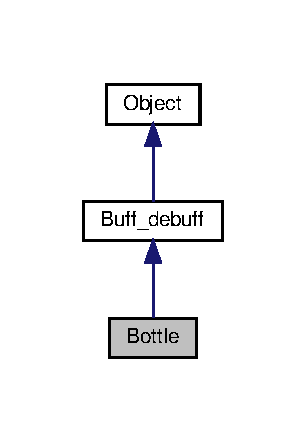
\includegraphics[width=147pt]{classBottle__inherit__graph}
\end{center}
\end{figure}


Collaboration diagram for Bottle\+:\nopagebreak
\begin{figure}[H]
\begin{center}
\leavevmode
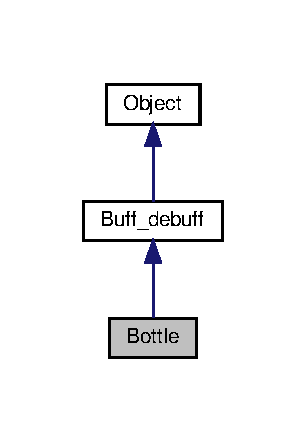
\includegraphics[width=147pt]{classBottle__coll__graph}
\end{center}
\end{figure}
\subsection*{Public Member Functions}
\begin{DoxyCompactItemize}
\item 
\hyperlink{classBottle_aabe46dbc52bfd8cf2a0088d96f86a767}{Bottle} (float, float)
\end{DoxyCompactItemize}
\subsection*{Additional Inherited Members}


\subsection{Detailed Description}
The bottle class creates a debuff object, bottle, that decreases the player speed when collided with. 

\subsection{Constructor \& Destructor Documentation}
\mbox{\Hypertarget{classBottle_aabe46dbc52bfd8cf2a0088d96f86a767}\label{classBottle_aabe46dbc52bfd8cf2a0088d96f86a767}} 
\index{Bottle@{Bottle}!Bottle@{Bottle}}
\index{Bottle@{Bottle}!Bottle@{Bottle}}
\subsubsection{\texorpdfstring{Bottle()}{Bottle()}}
{\footnotesize\ttfamily Bottle\+::\+Bottle (\begin{DoxyParamCaption}\item[{float}]{pos\+\_\+x,  }\item[{float}]{pos\+\_\+y }\end{DoxyParamCaption})}

The bottle constructor takes two float parameters, x-\/ and y-\/position(in that order). The constructor then loads the sprite for the bottle object, sets the scale for the sprite, sets the object position to the given parameters and sets the multiplier to 0.\+5. 

The documentation for this class was generated from the following files\+:\begin{DoxyCompactItemize}
\item 
buff\+\_\+debuff.\+h\item 
buff\+\_\+debuff.\+cpp\end{DoxyCompactItemize}

\hypertarget{classBuff__debuff}{}\section{Buff\+\_\+debuff Class Reference}
\label{classBuff__debuff}\index{Buff\+\_\+debuff@{Buff\+\_\+debuff}}


{\ttfamily \#include $<$buff\+\_\+debuff.\+h$>$}



Inheritance diagram for Buff\+\_\+debuff\+:\nopagebreak
\begin{figure}[H]
\begin{center}
\leavevmode
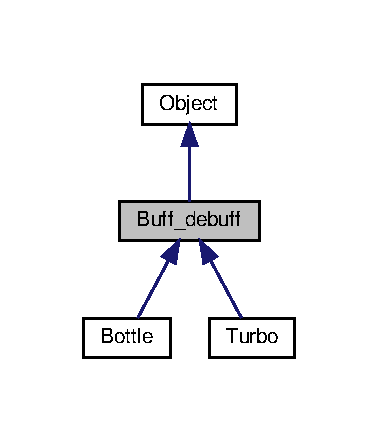
\includegraphics[width=182pt]{classBuff__debuff__inherit__graph}
\end{center}
\end{figure}


Collaboration diagram for Buff\+\_\+debuff\+:\nopagebreak
\begin{figure}[H]
\begin{center}
\leavevmode
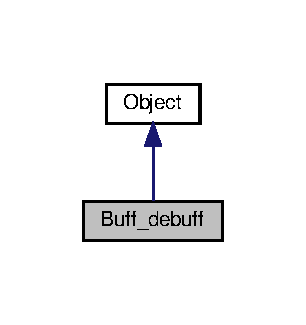
\includegraphics[width=147pt]{classBuff__debuff__coll__graph}
\end{center}
\end{figure}
\subsection*{Public Member Functions}
\begin{DoxyCompactItemize}
\item 
\hyperlink{classBuff__debuff_a7548567887d6e7f2280d488c800a098b}{Buff\+\_\+debuff} (float, float, float)
\item 
virtual \hyperlink{classBuff__debuff_a86ea03d85641f61757f121c6e226fafc}{$\sim$\+Buff\+\_\+debuff} ()=default
\item 
float \hyperlink{classBuff__debuff_ad72e20ee3b29b7ba11d36aa05a24f838}{get\+Multiplier} ()
\end{DoxyCompactItemize}
\subsection*{Protected Attributes}
\begin{DoxyCompactItemize}
\item 
float \hyperlink{classBuff__debuff_a0be49a0b6f19cb7cc160edad75109187}{multiplier} \{\}
\end{DoxyCompactItemize}


\subsection{Detailed Description}
Class \hyperlink{classBuff__debuff}{Buff\+\_\+debuff} is a parent class to the buff and the debuff classes \hyperlink{classTurbo}{Turbo} and \hyperlink{classBottle}{Bottle}. 

\subsection{Constructor \& Destructor Documentation}
\mbox{\Hypertarget{classBuff__debuff_a7548567887d6e7f2280d488c800a098b}\label{classBuff__debuff_a7548567887d6e7f2280d488c800a098b}} 
\index{Buff\+\_\+debuff@{Buff\+\_\+debuff}!Buff\+\_\+debuff@{Buff\+\_\+debuff}}
\index{Buff\+\_\+debuff@{Buff\+\_\+debuff}!Buff\+\_\+debuff@{Buff\+\_\+debuff}}
\subsubsection{\texorpdfstring{Buff\+\_\+debuff()}{Buff\_debuff()}}
{\footnotesize\ttfamily Buff\+\_\+debuff\+::\+Buff\+\_\+debuff (\begin{DoxyParamCaption}\item[{float}]{pos\+\_\+x,  }\item[{float}]{pos\+\_\+y,  }\item[{float}]{mult }\end{DoxyParamCaption})}

The \hyperlink{classBuff__debuff}{Buff\+\_\+debuff} constructor takes three floats as parameters. The first is the x-\/position of the buff, the second is the y-\/position of the buff relative to the gamefield, and the third is a multiplier that decides how the playerspeed is going to be affected. \mbox{\Hypertarget{classBuff__debuff_a86ea03d85641f61757f121c6e226fafc}\label{classBuff__debuff_a86ea03d85641f61757f121c6e226fafc}} 
\index{Buff\+\_\+debuff@{Buff\+\_\+debuff}!````~Buff\+\_\+debuff@{$\sim$\+Buff\+\_\+debuff}}
\index{````~Buff\+\_\+debuff@{$\sim$\+Buff\+\_\+debuff}!Buff\+\_\+debuff@{Buff\+\_\+debuff}}
\subsubsection{\texorpdfstring{$\sim$\+Buff\+\_\+debuff()}{~Buff\_debuff()}}
{\footnotesize\ttfamily virtual Buff\+\_\+debuff\+::$\sim$\+Buff\+\_\+debuff (\begin{DoxyParamCaption}{ }\end{DoxyParamCaption})\hspace{0.3cm}{\ttfamily [virtual]}, {\ttfamily [default]}}

The \hyperlink{classBuff__debuff}{Buff\+\_\+debuff} destructor is default. 

\subsection{Member Function Documentation}
\mbox{\Hypertarget{classBuff__debuff_ad72e20ee3b29b7ba11d36aa05a24f838}\label{classBuff__debuff_ad72e20ee3b29b7ba11d36aa05a24f838}} 
\index{Buff\+\_\+debuff@{Buff\+\_\+debuff}!get\+Multiplier@{get\+Multiplier}}
\index{get\+Multiplier@{get\+Multiplier}!Buff\+\_\+debuff@{Buff\+\_\+debuff}}
\subsubsection{\texorpdfstring{get\+Multiplier()}{getMultiplier()}}
{\footnotesize\ttfamily float Buff\+\_\+debuff\+::get\+Multiplier (\begin{DoxyParamCaption}{ }\end{DoxyParamCaption})}

Getter function that returns the protected member variable, multiplier. 

\subsection{Member Data Documentation}
\mbox{\Hypertarget{classBuff__debuff_a0be49a0b6f19cb7cc160edad75109187}\label{classBuff__debuff_a0be49a0b6f19cb7cc160edad75109187}} 
\index{Buff\+\_\+debuff@{Buff\+\_\+debuff}!multiplier@{multiplier}}
\index{multiplier@{multiplier}!Buff\+\_\+debuff@{Buff\+\_\+debuff}}
\subsubsection{\texorpdfstring{multiplier}{multiplier}}
{\footnotesize\ttfamily float Buff\+\_\+debuff\+::multiplier \{\}\hspace{0.3cm}{\ttfamily [protected]}}

Protected member variable that contains the multiplier that affects the player in case of collision with buff/debuff. 

The documentation for this class was generated from the following files\+:\begin{DoxyCompactItemize}
\item 
buff\+\_\+debuff.\+h\item 
buff\+\_\+debuff.\+cpp\end{DoxyCompactItemize}

\hypertarget{classBullet}{}\section{Bullet Class Reference}
\label{classBullet}\index{Bullet@{Bullet}}


{\ttfamily \#include $<$bullet.\+h$>$}



Inheritance diagram for Bullet\+:\nopagebreak
\begin{figure}[H]
\begin{center}
\leavevmode
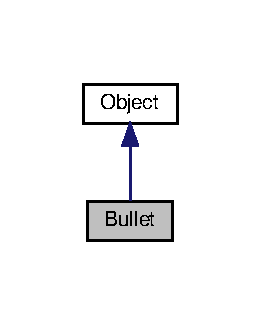
\includegraphics[width=125pt]{classBullet__inherit__graph}
\end{center}
\end{figure}


Collaboration diagram for Bullet\+:\nopagebreak
\begin{figure}[H]
\begin{center}
\leavevmode
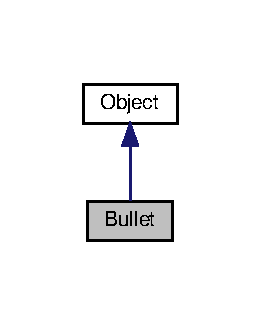
\includegraphics[width=125pt]{classBullet__coll__graph}
\end{center}
\end{figure}
\subsection*{Public Member Functions}
\begin{DoxyCompactItemize}
\item 
\hyperlink{classBullet_a5d934d668d3335e10f87302190608f57}{Bullet} (float, float)
\item 
\hyperlink{classBullet_a9e4f14ca4d33ad9445f13610135aa1f1}{$\sim$\+Bullet} ()=default
\end{DoxyCompactItemize}
\subsection*{Additional Inherited Members}


\subsection{Detailed Description}
The bullet class inherits from the object class as it creates a moving object in the game. This is the class that creates the projectile that is being shot when the player presses the spacebar. 

\subsection{Constructor \& Destructor Documentation}
\mbox{\Hypertarget{classBullet_a5d934d668d3335e10f87302190608f57}\label{classBullet_a5d934d668d3335e10f87302190608f57}} 
\index{Bullet@{Bullet}!Bullet@{Bullet}}
\index{Bullet@{Bullet}!Bullet@{Bullet}}
\subsubsection{\texorpdfstring{Bullet()}{Bullet()}}
{\footnotesize\ttfamily Bullet\+::\+Bullet (\begin{DoxyParamCaption}\item[{float}]{x,  }\item[{float}]{y }\end{DoxyParamCaption})}

The bullet constructor takes two float parameters, x-\/ and y-\/position(in that order). The constructor then loads the sprite for the bullet object, sets the scale for the sprite and sets position to the given parameters. \mbox{\Hypertarget{classBullet_a9e4f14ca4d33ad9445f13610135aa1f1}\label{classBullet_a9e4f14ca4d33ad9445f13610135aa1f1}} 
\index{Bullet@{Bullet}!````~Bullet@{$\sim$\+Bullet}}
\index{````~Bullet@{$\sim$\+Bullet}!Bullet@{Bullet}}
\subsubsection{\texorpdfstring{$\sim$\+Bullet()}{~Bullet()}}
{\footnotesize\ttfamily Bullet\+::$\sim$\+Bullet (\begin{DoxyParamCaption}{ }\end{DoxyParamCaption})\hspace{0.3cm}{\ttfamily [default]}}

The bullet destructor is default 

The documentation for this class was generated from the following files\+:\begin{DoxyCompactItemize}
\item 
bullet.\+h\item 
bullet.\+cpp\end{DoxyCompactItemize}

\hypertarget{classCar}{}\section{Car Class Reference}
\label{classCar}\index{Car@{Car}}


{\ttfamily \#include $<$car.\+h$>$}



Inheritance diagram for Car\+:\nopagebreak
\begin{figure}[H]
\begin{center}
\leavevmode
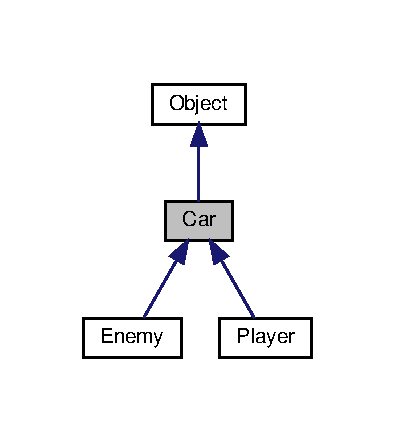
\includegraphics[width=190pt]{classCar__inherit__graph}
\end{center}
\end{figure}


Collaboration diagram for Car\+:\nopagebreak
\begin{figure}[H]
\begin{center}
\leavevmode
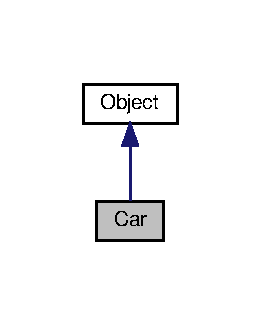
\includegraphics[width=125pt]{classCar__coll__graph}
\end{center}
\end{figure}
\subsection*{Public Member Functions}
\begin{DoxyCompactItemize}
\item 
\hyperlink{classCar_a1dd7bb5e39c21d7cc21fb5464dc6e397}{Car} (float, float)
\item 
virtual \hyperlink{classCar_a6d0e7bf36bd2588f9c119cf1b76d8e21}{$\sim$\+Car} ()=default
\item 
virtual void \hyperlink{classCar_a9650df764ceee00f738b888a7a976996}{car\+Move} (float, float)=0
\end{DoxyCompactItemize}
\subsection*{Protected Member Functions}
\begin{DoxyCompactItemize}
\item 
bool \hyperlink{classCar_a912e7849671d8390a9907917c0722549}{car\+Can\+Move} (float, float)
\end{DoxyCompactItemize}
\subsection*{Additional Inherited Members}


\subsection{Detailed Description}
Class Inherits from the \hyperlink{classObject}{Object} Class and acts as parent for \hyperlink{classPlayer}{Player} and \hyperlink{classEnemy}{Enemy} Class. 

\subsection{Constructor \& Destructor Documentation}
\mbox{\Hypertarget{classCar_a1dd7bb5e39c21d7cc21fb5464dc6e397}\label{classCar_a1dd7bb5e39c21d7cc21fb5464dc6e397}} 
\index{Car@{Car}!Car@{Car}}
\index{Car@{Car}!Car@{Car}}
\subsubsection{\texorpdfstring{Car()}{Car()}}
{\footnotesize\ttfamily Car\+::\+Car (\begin{DoxyParamCaption}\item[{float}]{pos\+\_\+x,  }\item[{float}]{pos\+\_\+y }\end{DoxyParamCaption})}

Constructor Takes 2 float parameters as car spawn position \mbox{\Hypertarget{classCar_a6d0e7bf36bd2588f9c119cf1b76d8e21}\label{classCar_a6d0e7bf36bd2588f9c119cf1b76d8e21}} 
\index{Car@{Car}!````~Car@{$\sim$\+Car}}
\index{````~Car@{$\sim$\+Car}!Car@{Car}}
\subsubsection{\texorpdfstring{$\sim$\+Car()}{~Car()}}
{\footnotesize\ttfamily virtual Car\+::$\sim$\+Car (\begin{DoxyParamCaption}{ }\end{DoxyParamCaption})\hspace{0.3cm}{\ttfamily [virtual]}, {\ttfamily [default]}}

Default destructor 

\subsection{Member Function Documentation}
\mbox{\Hypertarget{classCar_a912e7849671d8390a9907917c0722549}\label{classCar_a912e7849671d8390a9907917c0722549}} 
\index{Car@{Car}!car\+Can\+Move@{car\+Can\+Move}}
\index{car\+Can\+Move@{car\+Can\+Move}!Car@{Car}}
\subsubsection{\texorpdfstring{car\+Can\+Move()}{carCanMove()}}
{\footnotesize\ttfamily bool Car\+::car\+Can\+Move (\begin{DoxyParamCaption}\item[{float}]{new\+\_\+x,  }\item[{float}]{new\+\_\+y }\end{DoxyParamCaption})\hspace{0.3cm}{\ttfamily [protected]}}

Bool fuktion that checks if the \hyperlink{classCar}{Car} can move to the desired position. Takes two float parameters deciding where the car is trying to move. \mbox{\Hypertarget{classCar_a9650df764ceee00f738b888a7a976996}\label{classCar_a9650df764ceee00f738b888a7a976996}} 
\index{Car@{Car}!car\+Move@{car\+Move}}
\index{car\+Move@{car\+Move}!Car@{Car}}
\subsubsection{\texorpdfstring{car\+Move()}{carMove()}}
{\footnotesize\ttfamily virtual void Car\+::car\+Move (\begin{DoxyParamCaption}\item[{float}]{,  }\item[{float}]{ }\end{DoxyParamCaption})\hspace{0.3cm}{\ttfamily [pure virtual]}}

Virtual move funktion is specified in each class that inherits \hyperlink{classCar}{Car} 

Implemented in \hyperlink{classPlayer_a962661bbdff64b195582edbd0dcb3e1e}{Player}, and \hyperlink{classEnemy_a8b36ae5a6d6fd18d0064139ce92e7661}{Enemy}.



The documentation for this class was generated from the following files\+:\begin{DoxyCompactItemize}
\item 
car.\+h\item 
car.\+cpp\end{DoxyCompactItemize}

\hypertarget{classCollision}{}\section{Collision Class Reference}
\label{classCollision}\index{Collision@{Collision}}


{\ttfamily \#include $<$collision.\+h$>$}

\subsection*{Public Member Functions}
\begin{DoxyCompactItemize}
\item 
\hyperlink{classCollision_aea8004fbf48b79b5db7b784688b23788}{Collision} ()
\item 
bool \hyperlink{classCollision_a850f6ea5287cf6b2dd6765f5f9684cd5}{player\+\_\+enemy\+\_\+collide} (\hyperlink{classPlayer}{Player} \&, \hyperlink{classEnemy}{Enemy} \&)
\item 
bool \hyperlink{classCollision_ace87dc1e8d64435fda445f324b41fd58}{player\+\_\+buff\+\_\+debuff\+\_\+collide} (\hyperlink{classPlayer}{Player} \&, \hyperlink{classBuff__debuff}{Buff\+\_\+debuff} \&, sf\+::\+Time)
\item 
bool \hyperlink{classCollision_a3dcc2e9cfec6cc09445681a14fd3bfe4}{destroy\+At\+Bottom} (sf\+::\+Sprite)
\item 
bool \hyperlink{classCollision_a0a0e86390b15d8d745de4cf3707ced9d}{destroy\+At\+Top} (sf\+::\+Sprite)
\item 
bool \hyperlink{classCollision_a213b32a24bb00368732cd7170049c65e}{bullet\+\_\+enemy\+\_\+collide} (\hyperlink{classBullet}{Bullet} \&, \hyperlink{classEnemy}{Enemy} \&)
\end{DoxyCompactItemize}


\subsection{Detailed Description}
The role of the collision class is to check if the active objects on the screen are colliding with each other. The collision class interacts with the \hyperlink{classCar}{Car} class and also with its children player and enemy. This class also interacts with the \hyperlink{classBuff__debuff}{Buff\+\_\+debuff} class and it\textquotesingle{}s children \hyperlink{classTurbo}{Turbo} and \hyperlink{classBottle}{Bottle}. Lastly this class also interacts with the bullet class. 

\subsection{Constructor \& Destructor Documentation}
\mbox{\Hypertarget{classCollision_aea8004fbf48b79b5db7b784688b23788}\label{classCollision_aea8004fbf48b79b5db7b784688b23788}} 
\index{Collision@{Collision}!Collision@{Collision}}
\index{Collision@{Collision}!Collision@{Collision}}
\subsubsection{\texorpdfstring{Collision()}{Collision()}}
{\footnotesize\ttfamily Collision\+::\+Collision (\begin{DoxyParamCaption}{ }\end{DoxyParamCaption})\hspace{0.3cm}{\ttfamily [inline]}}

The collision constructor has no particular role, it is only needed to create a collision object that can be used to call the different collision functions. 

\subsection{Member Function Documentation}
\mbox{\Hypertarget{classCollision_a213b32a24bb00368732cd7170049c65e}\label{classCollision_a213b32a24bb00368732cd7170049c65e}} 
\index{Collision@{Collision}!bullet\+\_\+enemy\+\_\+collide@{bullet\+\_\+enemy\+\_\+collide}}
\index{bullet\+\_\+enemy\+\_\+collide@{bullet\+\_\+enemy\+\_\+collide}!Collision@{Collision}}
\subsubsection{\texorpdfstring{bullet\+\_\+enemy\+\_\+collide()}{bullet\_enemy\_collide()}}
{\footnotesize\ttfamily bool Collision\+::bullet\+\_\+enemy\+\_\+collide (\begin{DoxyParamCaption}\item[{\hyperlink{classBullet}{Bullet} \&}]{bullet,  }\item[{\hyperlink{classEnemy}{Enemy} \&}]{enemy }\end{DoxyParamCaption})}

Function takes a two object references, the first to the bullet object and the second to the enemy object. The function checks if the bullet global bounds are intersecting the enemy global bounds and returns a bool true if they do or a bool false if they don\textquotesingle{}t. \mbox{\Hypertarget{classCollision_a3dcc2e9cfec6cc09445681a14fd3bfe4}\label{classCollision_a3dcc2e9cfec6cc09445681a14fd3bfe4}} 
\index{Collision@{Collision}!destroy\+At\+Bottom@{destroy\+At\+Bottom}}
\index{destroy\+At\+Bottom@{destroy\+At\+Bottom}!Collision@{Collision}}
\subsubsection{\texorpdfstring{destroy\+At\+Bottom()}{destroyAtBottom()}}
{\footnotesize\ttfamily bool Collision\+::destroy\+At\+Bottom (\begin{DoxyParamCaption}\item[{sf\+::\+Sprite}]{shape }\end{DoxyParamCaption})}

Checks if sprite position is equal to or less than 8 pixels from the bottom. Returns true if it is. \mbox{\Hypertarget{classCollision_a0a0e86390b15d8d745de4cf3707ced9d}\label{classCollision_a0a0e86390b15d8d745de4cf3707ced9d}} 
\index{Collision@{Collision}!destroy\+At\+Top@{destroy\+At\+Top}}
\index{destroy\+At\+Top@{destroy\+At\+Top}!Collision@{Collision}}
\subsubsection{\texorpdfstring{destroy\+At\+Top()}{destroyAtTop()}}
{\footnotesize\ttfamily bool Collision\+::destroy\+At\+Top (\begin{DoxyParamCaption}\item[{sf\+::\+Sprite}]{shape }\end{DoxyParamCaption})}

Checks if the sprite position is equal to or less than 8 pixels from the top. Returns true if it is. \mbox{\Hypertarget{classCollision_ace87dc1e8d64435fda445f324b41fd58}\label{classCollision_ace87dc1e8d64435fda445f324b41fd58}} 
\index{Collision@{Collision}!player\+\_\+buff\+\_\+debuff\+\_\+collide@{player\+\_\+buff\+\_\+debuff\+\_\+collide}}
\index{player\+\_\+buff\+\_\+debuff\+\_\+collide@{player\+\_\+buff\+\_\+debuff\+\_\+collide}!Collision@{Collision}}
\subsubsection{\texorpdfstring{player\+\_\+buff\+\_\+debuff\+\_\+collide()}{player\_buff\_debuff\_collide()}}
{\footnotesize\ttfamily bool Collision\+::player\+\_\+buff\+\_\+debuff\+\_\+collide (\begin{DoxyParamCaption}\item[{\hyperlink{classPlayer}{Player} \&}]{player,  }\item[{\hyperlink{classBuff__debuff}{Buff\+\_\+debuff} \&}]{buff\+\_\+debuff,  }\item[{sf\+::\+Time}]{player\+\_\+state\+\_\+time }\end{DoxyParamCaption})}

Function takes three parameters. The first is a reference to a player object, the second is a reference to a buff or debuff object and the third is an sf\+::\+Time object. The function checks if the global bound of the two objects intersect. If the object intersect, the player multiplier is changed to that of the buff/debuff, the player variable state\+Is\+Changed is changed to true if it is not already that and ten seconds are added to the player variable state\+Time during which the player is affected by the buff. The player state is changed everytime there is a collision between these objects. If the player state is already changed then the new collision will reset the timer to ten seconds and apply the multiplier relative to the player base speed not current one. \mbox{\Hypertarget{classCollision_a850f6ea5287cf6b2dd6765f5f9684cd5}\label{classCollision_a850f6ea5287cf6b2dd6765f5f9684cd5}} 
\index{Collision@{Collision}!player\+\_\+enemy\+\_\+collide@{player\+\_\+enemy\+\_\+collide}}
\index{player\+\_\+enemy\+\_\+collide@{player\+\_\+enemy\+\_\+collide}!Collision@{Collision}}
\subsubsection{\texorpdfstring{player\+\_\+enemy\+\_\+collide()}{player\_enemy\_collide()}}
{\footnotesize\ttfamily bool Collision\+::player\+\_\+enemy\+\_\+collide (\begin{DoxyParamCaption}\item[{\hyperlink{classPlayer}{Player} \&}]{player,  }\item[{\hyperlink{classEnemy}{Enemy} \&}]{enemy }\end{DoxyParamCaption})}

Function takes a two object references, the first to the player object and the second to the enemy object. The function checks if the player global bounds are intersecting the enemy global bounds and returns a bool true if they do or a bool false if they don\textquotesingle{}t. 

The documentation for this class was generated from the following files\+:\begin{DoxyCompactItemize}
\item 
collision.\+h\item 
collision.\+cpp\end{DoxyCompactItemize}

\hypertarget{classEnemy}{}\section{Enemy Class Reference}
\label{classEnemy}\index{Enemy@{Enemy}}


{\ttfamily \#include $<$car.\+h$>$}



Inheritance diagram for Enemy\+:\nopagebreak
\begin{figure}[H]
\begin{center}
\leavevmode
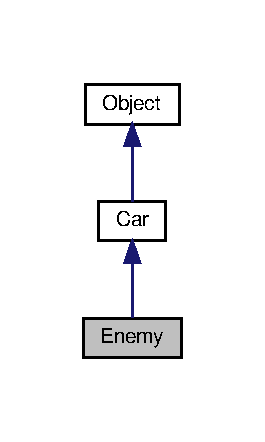
\includegraphics[width=127pt]{classEnemy__inherit__graph}
\end{center}
\end{figure}


Collaboration diagram for Enemy\+:\nopagebreak
\begin{figure}[H]
\begin{center}
\leavevmode
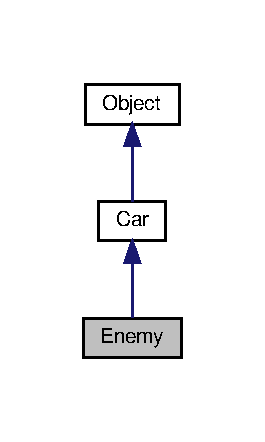
\includegraphics[width=127pt]{classEnemy__coll__graph}
\end{center}
\end{figure}
\subsection*{Public Member Functions}
\begin{DoxyCompactItemize}
\item 
\hyperlink{classEnemy_a3aca7827da68a391100d2bc1a4873625}{Enemy} (float, float)
\item 
void \hyperlink{classEnemy_a8b36ae5a6d6fd18d0064139ce92e7661}{car\+Move} (float, float)
\item 
void \hyperlink{classEnemy_a58402ae6b3e519ecad7d1c61961a4904}{change\+Lane} ()
\end{DoxyCompactItemize}
\subsection*{Public Attributes}
\begin{DoxyCompactItemize}
\item 
bool \hyperlink{classEnemy_a2d4bfba6681a78723c61c284a5e1f2d5}{is\+Moving\+Left} \{false\}
\item 
bool \hyperlink{classEnemy_a69ab0772337c6de349a6a412d10876e7}{is\+Moving\+Right} \{false\}
\end{DoxyCompactItemize}
\subsection*{Additional Inherited Members}


\subsection{Detailed Description}
Class Represents the enemies in the game. 

\subsection{Constructor \& Destructor Documentation}
\mbox{\Hypertarget{classEnemy_a3aca7827da68a391100d2bc1a4873625}\label{classEnemy_a3aca7827da68a391100d2bc1a4873625}} 
\index{Enemy@{Enemy}!Enemy@{Enemy}}
\index{Enemy@{Enemy}!Enemy@{Enemy}}
\subsubsection{\texorpdfstring{Enemy()}{Enemy()}}
{\footnotesize\ttfamily Enemy\+::\+Enemy (\begin{DoxyParamCaption}\item[{float}]{pos\+\_\+x,  }\item[{float}]{pos\+\_\+y }\end{DoxyParamCaption})}

Loads the specified sprite for \hyperlink{classEnemy}{Enemy} and saves it. 

\subsection{Member Function Documentation}
\mbox{\Hypertarget{classEnemy_a8b36ae5a6d6fd18d0064139ce92e7661}\label{classEnemy_a8b36ae5a6d6fd18d0064139ce92e7661}} 
\index{Enemy@{Enemy}!car\+Move@{car\+Move}}
\index{car\+Move@{car\+Move}!Enemy@{Enemy}}
\subsubsection{\texorpdfstring{car\+Move()}{carMove()}}
{\footnotesize\ttfamily void Enemy\+::car\+Move (\begin{DoxyParamCaption}\item[{float}]{x,  }\item[{float}]{y }\end{DoxyParamCaption})\hspace{0.3cm}{\ttfamily [virtual]}}

Specifik car\+Move funktion 

Implements \hyperlink{classCar_a9650df764ceee00f738b888a7a976996}{Car}.

\mbox{\Hypertarget{classEnemy_a58402ae6b3e519ecad7d1c61961a4904}\label{classEnemy_a58402ae6b3e519ecad7d1c61961a4904}} 
\index{Enemy@{Enemy}!change\+Lane@{change\+Lane}}
\index{change\+Lane@{change\+Lane}!Enemy@{Enemy}}
\subsubsection{\texorpdfstring{change\+Lane()}{changeLane()}}
{\footnotesize\ttfamily void Enemy\+::change\+Lane (\begin{DoxyParamCaption}{ }\end{DoxyParamCaption})}

Changes \hyperlink{classEnemy}{Enemy} position on the x axle depending on the bool variables is\+Moving\+Left and is\+Moving\+Right. 

\subsection{Member Data Documentation}
\mbox{\Hypertarget{classEnemy_a2d4bfba6681a78723c61c284a5e1f2d5}\label{classEnemy_a2d4bfba6681a78723c61c284a5e1f2d5}} 
\index{Enemy@{Enemy}!is\+Moving\+Left@{is\+Moving\+Left}}
\index{is\+Moving\+Left@{is\+Moving\+Left}!Enemy@{Enemy}}
\subsubsection{\texorpdfstring{is\+Moving\+Left}{isMovingLeft}}
{\footnotesize\ttfamily bool Enemy\+::is\+Moving\+Left \{false\}}

Shows if the \hyperlink{classEnemy}{Enemy} should be moving left or not \mbox{\Hypertarget{classEnemy_a69ab0772337c6de349a6a412d10876e7}\label{classEnemy_a69ab0772337c6de349a6a412d10876e7}} 
\index{Enemy@{Enemy}!is\+Moving\+Right@{is\+Moving\+Right}}
\index{is\+Moving\+Right@{is\+Moving\+Right}!Enemy@{Enemy}}
\subsubsection{\texorpdfstring{is\+Moving\+Right}{isMovingRight}}
{\footnotesize\ttfamily bool Enemy\+::is\+Moving\+Right \{false\}}

Shows if the \hyperlink{classEnemy}{Enemy} should be moving right or not 

The documentation for this class was generated from the following files\+:\begin{DoxyCompactItemize}
\item 
car.\+h\item 
car.\+cpp\end{DoxyCompactItemize}

\hypertarget{classGame}{}\section{Game Class Reference}
\label{classGame}\index{Game@{Game}}


{\ttfamily \#include $<$game\+\_\+state.\+h$>$}

\subsection*{Public Member Functions}
\begin{DoxyCompactItemize}
\item 
\hyperlink{classGame_a071ee8ba1e8d3874d369571fc21b1628}{Game} (sf\+::\+Render\+Window \&)
\item 
int \hyperlink{classGame_a99fb161fbbe87d25a8b73265a0611e58}{run} ()
\item 
\hyperlink{classGame_ae3d112ca6e0e55150d2fdbc704474530}{$\sim$\+Game} ()
\end{DoxyCompactItemize}


\subsection{Detailed Description}
Class Represents the \hyperlink{classGame}{Game} and holds all needed game objects. 

\subsection{Constructor \& Destructor Documentation}
\mbox{\Hypertarget{classGame_a071ee8ba1e8d3874d369571fc21b1628}\label{classGame_a071ee8ba1e8d3874d369571fc21b1628}} 
\index{Game@{Game}!Game@{Game}}
\index{Game@{Game}!Game@{Game}}
\subsubsection{\texorpdfstring{Game()}{Game()}}
{\footnotesize\ttfamily Game\+::\+Game (\begin{DoxyParamCaption}\item[{sf\+::\+Render\+Window \&}]{win }\end{DoxyParamCaption})}

Takes a Render\+Window parameter to wich it sets the window variable to. \mbox{\Hypertarget{classGame_ae3d112ca6e0e55150d2fdbc704474530}\label{classGame_ae3d112ca6e0e55150d2fdbc704474530}} 
\index{Game@{Game}!````~Game@{$\sim$\+Game}}
\index{````~Game@{$\sim$\+Game}!Game@{Game}}
\subsubsection{\texorpdfstring{$\sim$\+Game()}{~Game()}}
{\footnotesize\ttfamily Game\+::$\sim$\+Game (\begin{DoxyParamCaption}{ }\end{DoxyParamCaption})}

Deletes all objects saved on the heap. 

\subsection{Member Function Documentation}
\mbox{\Hypertarget{classGame_a99fb161fbbe87d25a8b73265a0611e58}\label{classGame_a99fb161fbbe87d25a8b73265a0611e58}} 
\index{Game@{Game}!run@{run}}
\index{run@{run}!Game@{Game}}
\subsubsection{\texorpdfstring{run()}{run()}}
{\footnotesize\ttfamily int Game\+::run (\begin{DoxyParamCaption}{ }\end{DoxyParamCaption})}

Runs the game loop. 

The documentation for this class was generated from the following files\+:\begin{DoxyCompactItemize}
\item 
game\+\_\+state.\+h\item 
game\+\_\+state.\+cpp\end{DoxyCompactItemize}

\hypertarget{classGame__Field}{}\section{Game\+\_\+\+Field Class Reference}
\label{classGame__Field}\index{Game\+\_\+\+Field@{Game\+\_\+\+Field}}


{\ttfamily \#include $<$game\+\_\+field.\+h$>$}

\subsection*{Public Member Functions}
\begin{DoxyCompactItemize}
\item 
\hyperlink{classGame__Field_aa62311d75d2c83c069535ca310b7585d}{Game\+\_\+\+Field} ()
\item 
\hyperlink{classGame__Field_a1cc20d15758ae0d3e31492448bc4d47f}{$\sim$\+Game\+\_\+\+Field} ()
\item 
std\+::vector$<$ sf\+::\+Texture $\ast$ $>$ \hyperlink{classGame__Field_ad2f37858f33af0caf2cd4ba0107a9a24}{load} ()
\item 
void \hyperlink{classGame__Field_a60de25cfcba5f7f67a5bf510cdc13326}{display} (sf\+::\+Render\+Window \&)
\item 
int \hyperlink{classGame__Field_a2a328d2a97c5f90a2cd35a89e1cedb01}{enemy\+\_\+spawn} ()
\item 
int \hyperlink{classGame__Field_a8f7d0feefd13f9ba229e08d4e270528d}{buff\+\_\+spawn} ()
\item 
float \hyperlink{classGame__Field_a6ccee168fe4ca574f3b9de452cecc38c}{x\+\_\+spawn} ()
\item 
int \hyperlink{classGame__Field_ae174d69a829b073c9b64e9f15e57870d}{enemy\+\_\+move} ()
\end{DoxyCompactItemize}
\subsection*{Public Attributes}
\begin{DoxyCompactItemize}
\item 
int \hyperlink{classGame__Field_a3d3cda2cf3a0eae2229f5b4a6e0ae532}{loop\+\_\+speed} \{3\}
\end{DoxyCompactItemize}


\subsection{Detailed Description}
Class Takes care of spawn probability, and the background loop. 

\subsection{Constructor \& Destructor Documentation}
\mbox{\Hypertarget{classGame__Field_aa62311d75d2c83c069535ca310b7585d}\label{classGame__Field_aa62311d75d2c83c069535ca310b7585d}} 
\index{Game\+\_\+\+Field@{Game\+\_\+\+Field}!Game\+\_\+\+Field@{Game\+\_\+\+Field}}
\index{Game\+\_\+\+Field@{Game\+\_\+\+Field}!Game\+\_\+\+Field@{Game\+\_\+\+Field}}
\subsubsection{\texorpdfstring{Game\+\_\+\+Field()}{Game\_Field()}}
{\footnotesize\ttfamily Game\+\_\+\+Field\+::\+Game\+\_\+\+Field (\begin{DoxyParamCaption}{ }\end{DoxyParamCaption})}

Starts the load function for the background \mbox{\Hypertarget{classGame__Field_a1cc20d15758ae0d3e31492448bc4d47f}\label{classGame__Field_a1cc20d15758ae0d3e31492448bc4d47f}} 
\index{Game\+\_\+\+Field@{Game\+\_\+\+Field}!````~Game\+\_\+\+Field@{$\sim$\+Game\+\_\+\+Field}}
\index{````~Game\+\_\+\+Field@{$\sim$\+Game\+\_\+\+Field}!Game\+\_\+\+Field@{Game\+\_\+\+Field}}
\subsubsection{\texorpdfstring{$\sim$\+Game\+\_\+\+Field()}{~Game\_Field()}}
{\footnotesize\ttfamily Game\+\_\+\+Field\+::$\sim$\+Game\+\_\+\+Field (\begin{DoxyParamCaption}{ }\end{DoxyParamCaption})}

Deletes all the textures for the background 

\subsection{Member Function Documentation}
\mbox{\Hypertarget{classGame__Field_a8f7d0feefd13f9ba229e08d4e270528d}\label{classGame__Field_a8f7d0feefd13f9ba229e08d4e270528d}} 
\index{Game\+\_\+\+Field@{Game\+\_\+\+Field}!buff\+\_\+spawn@{buff\+\_\+spawn}}
\index{buff\+\_\+spawn@{buff\+\_\+spawn}!Game\+\_\+\+Field@{Game\+\_\+\+Field}}
\subsubsection{\texorpdfstring{buff\+\_\+spawn()}{buff\_spawn()}}
{\footnotesize\ttfamily int Game\+\_\+\+Field\+::buff\+\_\+spawn (\begin{DoxyParamCaption}{ }\end{DoxyParamCaption})}

Returns an int for deciding if a \hyperlink{classTurbo}{Turbo} or \hyperlink{classBottle}{Bottle} should spawn. \mbox{\Hypertarget{classGame__Field_a60de25cfcba5f7f67a5bf510cdc13326}\label{classGame__Field_a60de25cfcba5f7f67a5bf510cdc13326}} 
\index{Game\+\_\+\+Field@{Game\+\_\+\+Field}!display@{display}}
\index{display@{display}!Game\+\_\+\+Field@{Game\+\_\+\+Field}}
\subsubsection{\texorpdfstring{display()}{display()}}
{\footnotesize\ttfamily void Game\+\_\+\+Field\+::display (\begin{DoxyParamCaption}\item[{sf\+::\+Render\+Window \&}]{window }\end{DoxyParamCaption})}

Displays the current index of the background loop to the window parameter. \mbox{\Hypertarget{classGame__Field_ae174d69a829b073c9b64e9f15e57870d}\label{classGame__Field_ae174d69a829b073c9b64e9f15e57870d}} 
\index{Game\+\_\+\+Field@{Game\+\_\+\+Field}!enemy\+\_\+move@{enemy\+\_\+move}}
\index{enemy\+\_\+move@{enemy\+\_\+move}!Game\+\_\+\+Field@{Game\+\_\+\+Field}}
\subsubsection{\texorpdfstring{enemy\+\_\+move()}{enemy\_move()}}
{\footnotesize\ttfamily int Game\+\_\+\+Field\+::enemy\+\_\+move (\begin{DoxyParamCaption}{ }\end{DoxyParamCaption})}

Returns an int for deciding if a \hyperlink{classEnemy}{Enemy} should move. \mbox{\Hypertarget{classGame__Field_a2a328d2a97c5f90a2cd35a89e1cedb01}\label{classGame__Field_a2a328d2a97c5f90a2cd35a89e1cedb01}} 
\index{Game\+\_\+\+Field@{Game\+\_\+\+Field}!enemy\+\_\+spawn@{enemy\+\_\+spawn}}
\index{enemy\+\_\+spawn@{enemy\+\_\+spawn}!Game\+\_\+\+Field@{Game\+\_\+\+Field}}
\subsubsection{\texorpdfstring{enemy\+\_\+spawn()}{enemy\_spawn()}}
{\footnotesize\ttfamily int Game\+\_\+\+Field\+::enemy\+\_\+spawn (\begin{DoxyParamCaption}{ }\end{DoxyParamCaption})}

Returns an int for deciding if a \hyperlink{classEnemy}{Enemy} should spawn. \mbox{\Hypertarget{classGame__Field_ad2f37858f33af0caf2cd4ba0107a9a24}\label{classGame__Field_ad2f37858f33af0caf2cd4ba0107a9a24}} 
\index{Game\+\_\+\+Field@{Game\+\_\+\+Field}!load@{load}}
\index{load@{load}!Game\+\_\+\+Field@{Game\+\_\+\+Field}}
\subsubsection{\texorpdfstring{load()}{load()}}
{\footnotesize\ttfamily std\+::vector$<$ sf\+::\+Texture $\ast$ $>$ Game\+\_\+\+Field\+::load (\begin{DoxyParamCaption}{ }\end{DoxyParamCaption})}

Loads all the background textures and saves pointers to them in a vector, which it then returns. \mbox{\Hypertarget{classGame__Field_a6ccee168fe4ca574f3b9de452cecc38c}\label{classGame__Field_a6ccee168fe4ca574f3b9de452cecc38c}} 
\index{Game\+\_\+\+Field@{Game\+\_\+\+Field}!x\+\_\+spawn@{x\+\_\+spawn}}
\index{x\+\_\+spawn@{x\+\_\+spawn}!Game\+\_\+\+Field@{Game\+\_\+\+Field}}
\subsubsection{\texorpdfstring{x\+\_\+spawn()}{x\_spawn()}}
{\footnotesize\ttfamily float Game\+\_\+\+Field\+::x\+\_\+spawn (\begin{DoxyParamCaption}{ }\end{DoxyParamCaption})}

Returns a float representing an Objects x spawn value. 

\subsection{Member Data Documentation}
\mbox{\Hypertarget{classGame__Field_a3d3cda2cf3a0eae2229f5b4a6e0ae532}\label{classGame__Field_a3d3cda2cf3a0eae2229f5b4a6e0ae532}} 
\index{Game\+\_\+\+Field@{Game\+\_\+\+Field}!loop\+\_\+speed@{loop\+\_\+speed}}
\index{loop\+\_\+speed@{loop\+\_\+speed}!Game\+\_\+\+Field@{Game\+\_\+\+Field}}
\subsubsection{\texorpdfstring{loop\+\_\+speed}{loop\_speed}}
{\footnotesize\ttfamily int Game\+\_\+\+Field\+::loop\+\_\+speed \{3\}}

Represents the current loop speed for the display function. 

The documentation for this class was generated from the following files\+:\begin{DoxyCompactItemize}
\item 
game\+\_\+field.\+h\item 
game\+\_\+field.\+cpp\end{DoxyCompactItemize}

\hypertarget{classMenu}{}\section{Menu Class Reference}
\label{classMenu}\index{Menu@{Menu}}


{\ttfamily \#include $<$menu\+\_\+state.\+h$>$}

\subsection*{Public Member Functions}
\begin{DoxyCompactItemize}
\item 
\hyperlink{classMenu_aff5b4e8e5376fec2d1929bfb30f802ed}{Menu} (sf\+::\+Render\+Window \&)
\item 
int \hyperlink{classMenu_af93a970cdfec463a8cb25ca65bf51da5}{run} ()
\item 
void \hyperlink{classMenu_a2cd7ab9901a8f42a3ae977d0774398a6}{draw} ()
\item 
void \hyperlink{classMenu_abfa1619b1d868d85b3978f5918c2a56f}{move\+Up} ()
\item 
void \hyperlink{classMenu_abbec620bd41608fba287400ead4467aa}{move\+Down} ()
\item 
void \hyperlink{classMenu_a9516e2d4872c03ba5a436216d1729e35}{set\+Score} (int)
\item 
int \hyperlink{classMenu_a6cb35aed2a232dcc0859c3b4e419454c}{get\+Pressed\+Item} ()
\end{DoxyCompactItemize}
\subsection*{Public Attributes}
\begin{DoxyCompactItemize}
\item 
sf\+::\+Render\+Window \& \hyperlink{classMenu_a56a1907bf19e3ccdfbd31189c71fc18c}{window}
\item 
int \hyperlink{classMenu_a7e426cd425c8d7e898c6b80e59339e5f}{score} \{0\}
\end{DoxyCompactItemize}


\subsection{Detailed Description}
The menu class is the class that handles showing the menu, the game over screen and that starts the game. 

\subsection{Constructor \& Destructor Documentation}
\mbox{\Hypertarget{classMenu_aff5b4e8e5376fec2d1929bfb30f802ed}\label{classMenu_aff5b4e8e5376fec2d1929bfb30f802ed}} 
\index{Menu@{Menu}!Menu@{Menu}}
\index{Menu@{Menu}!Menu@{Menu}}
\subsubsection{\texorpdfstring{Menu()}{Menu()}}
{\footnotesize\ttfamily Menu\+::\+Menu (\begin{DoxyParamCaption}\item[{sf\+::\+Render\+Window \&}]{window }\end{DoxyParamCaption})}

The constructor takes a reference to an sf\+::\+Render\+Window to get it\textquotesingle{}s width and height. It proceeds to create three elements that are storred in the private variable menu. The first is a text that shows the score(that is not being shown before the game runs), the second is a play button and the third is an exit button. With the width and height of the window the elements are being centered in the picture. 

\subsection{Member Function Documentation}
\mbox{\Hypertarget{classMenu_a2cd7ab9901a8f42a3ae977d0774398a6}\label{classMenu_a2cd7ab9901a8f42a3ae977d0774398a6}} 
\index{Menu@{Menu}!draw@{draw}}
\index{draw@{draw}!Menu@{Menu}}
\subsubsection{\texorpdfstring{draw()}{draw()}}
{\footnotesize\ttfamily void Menu\+::draw (\begin{DoxyParamCaption}{ }\end{DoxyParamCaption})}

Loops through the array that contains all the elements and draws two of them if it is run before the game or draws all three if it runs after the game has run. \mbox{\Hypertarget{classMenu_a6cb35aed2a232dcc0859c3b4e419454c}\label{classMenu_a6cb35aed2a232dcc0859c3b4e419454c}} 
\index{Menu@{Menu}!get\+Pressed\+Item@{get\+Pressed\+Item}}
\index{get\+Pressed\+Item@{get\+Pressed\+Item}!Menu@{Menu}}
\subsubsection{\texorpdfstring{get\+Pressed\+Item()}{getPressedItem()}}
{\footnotesize\ttfamily int Menu\+::get\+Pressed\+Item (\begin{DoxyParamCaption}{ }\end{DoxyParamCaption})}

Returns selected\+Item\+Index to find out which button was being pressed. \mbox{\Hypertarget{classMenu_abbec620bd41608fba287400ead4467aa}\label{classMenu_abbec620bd41608fba287400ead4467aa}} 
\index{Menu@{Menu}!move\+Down@{move\+Down}}
\index{move\+Down@{move\+Down}!Menu@{Menu}}
\subsubsection{\texorpdfstring{move\+Down()}{moveDown()}}
{\footnotesize\ttfamily void Menu\+::move\+Down (\begin{DoxyParamCaption}{ }\end{DoxyParamCaption})}

Adds to the selected\+Item\+Index variable and changes the menu text colors to give the illusion that the player moves down in the menu. \mbox{\Hypertarget{classMenu_abfa1619b1d868d85b3978f5918c2a56f}\label{classMenu_abfa1619b1d868d85b3978f5918c2a56f}} 
\index{Menu@{Menu}!move\+Up@{move\+Up}}
\index{move\+Up@{move\+Up}!Menu@{Menu}}
\subsubsection{\texorpdfstring{move\+Up()}{moveUp()}}
{\footnotesize\ttfamily void Menu\+::move\+Up (\begin{DoxyParamCaption}{ }\end{DoxyParamCaption})}

Subtracts from the selected\+Item\+Index variable and changes the menu text colors to give the illusion that the player moves up in the menu. \mbox{\Hypertarget{classMenu_af93a970cdfec463a8cb25ca65bf51da5}\label{classMenu_af93a970cdfec463a8cb25ca65bf51da5}} 
\index{Menu@{Menu}!run@{run}}
\index{run@{run}!Menu@{Menu}}
\subsubsection{\texorpdfstring{run()}{run()}}
{\footnotesize\ttfamily int Menu\+::run (\begin{DoxyParamCaption}{ }\end{DoxyParamCaption})}

The function that runs the menu loop that checks for buttons being pressed, sets the string score that needs to be displayed, draws and displays the menu. \mbox{\Hypertarget{classMenu_a9516e2d4872c03ba5a436216d1729e35}\label{classMenu_a9516e2d4872c03ba5a436216d1729e35}} 
\index{Menu@{Menu}!set\+Score@{set\+Score}}
\index{set\+Score@{set\+Score}!Menu@{Menu}}
\subsubsection{\texorpdfstring{set\+Score()}{setScore()}}
{\footnotesize\ttfamily void Menu\+::set\+Score (\begin{DoxyParamCaption}\item[{int}]{the\+\_\+score }\end{DoxyParamCaption})}

Setter function that sets the score variable. This is the variable that is later displayed as the score. 

\subsection{Member Data Documentation}
\mbox{\Hypertarget{classMenu_a7e426cd425c8d7e898c6b80e59339e5f}\label{classMenu_a7e426cd425c8d7e898c6b80e59339e5f}} 
\index{Menu@{Menu}!score@{score}}
\index{score@{score}!Menu@{Menu}}
\subsubsection{\texorpdfstring{score}{score}}
{\footnotesize\ttfamily int Menu\+::score \{0\}}

Int variable that contains the score that is being returned from the gamestate. It is 0 as standard. \mbox{\Hypertarget{classMenu_a56a1907bf19e3ccdfbd31189c71fc18c}\label{classMenu_a56a1907bf19e3ccdfbd31189c71fc18c}} 
\index{Menu@{Menu}!window@{window}}
\index{window@{window}!Menu@{Menu}}
\subsubsection{\texorpdfstring{window}{window}}
{\footnotesize\ttfamily sf\+::\+Render\+Window\& Menu\+::window}

Public variable that contains a window object where everything is being drawn. 

The documentation for this class was generated from the following files\+:\begin{DoxyCompactItemize}
\item 
menu\+\_\+state.\+h\item 
menu\+\_\+state.\+cpp\end{DoxyCompactItemize}

\hypertarget{classObject}{}\section{Object Class Reference}
\label{classObject}\index{Object@{Object}}


{\ttfamily \#include $<$object.\+h$>$}



Inheritance diagram for Object\+:\nopagebreak
\begin{figure}[H]
\begin{center}
\leavevmode
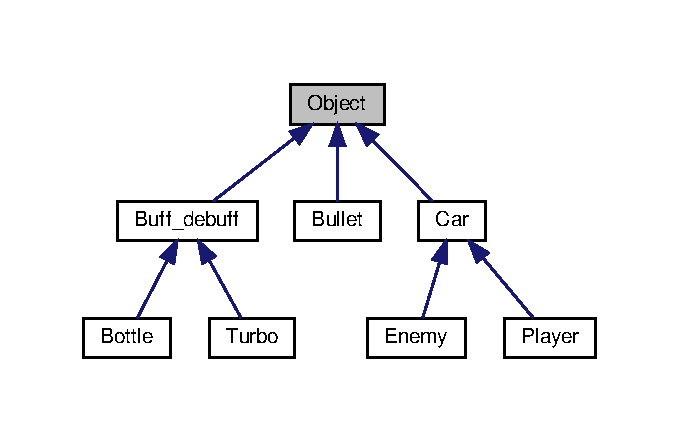
\includegraphics[width=326pt]{classObject__inherit__graph}
\end{center}
\end{figure}
\subsection*{Public Member Functions}
\begin{DoxyCompactItemize}
\item 
void \hyperlink{classObject_a9e90592420891436fef1a41c42498e8b}{draw} (sf\+::\+Render\+Window \&)
\item 
sf\+::\+Sprite \hyperlink{classObject_ae38e77de9a92daab0e6fea8d3ba56fdd}{get\+Shape} ()
\item 
void \hyperlink{classObject_a2cded255e6f55fb4542ca036450876f3}{move} (float, float)
\end{DoxyCompactItemize}
\subsection*{Protected Attributes}
\begin{DoxyCompactItemize}
\item 
sf\+::\+Texture \hyperlink{classObject_a8abc6192982ee39b2dc9d9b05cc155ee}{texture}
\item 
sf\+::\+Sprite \hyperlink{classObject_a563c6c058bb3549ef8bc8cbc01c4e7e1}{shape}
\end{DoxyCompactItemize}


\subsection{Detailed Description}
Class Represents all active objects in the game. 

\subsection{Member Function Documentation}
\mbox{\Hypertarget{classObject_a9e90592420891436fef1a41c42498e8b}\label{classObject_a9e90592420891436fef1a41c42498e8b}} 
\index{Object@{Object}!draw@{draw}}
\index{draw@{draw}!Object@{Object}}
\subsubsection{\texorpdfstring{draw()}{draw()}}
{\footnotesize\ttfamily void Object\+::draw (\begin{DoxyParamCaption}\item[{sf\+::\+Render\+Window \&}]{window }\end{DoxyParamCaption})}

Draws the saved sprite \char`\"{}shape\char`\"{} to a Render\+Window refrence. \mbox{\Hypertarget{classObject_ae38e77de9a92daab0e6fea8d3ba56fdd}\label{classObject_ae38e77de9a92daab0e6fea8d3ba56fdd}} 
\index{Object@{Object}!get\+Shape@{get\+Shape}}
\index{get\+Shape@{get\+Shape}!Object@{Object}}
\subsubsection{\texorpdfstring{get\+Shape()}{getShape()}}
{\footnotesize\ttfamily sf\+::\+Sprite Object\+::get\+Shape (\begin{DoxyParamCaption}{ }\end{DoxyParamCaption})}

Returns the saved Sprite \char`\"{}shape\char`\"{}. \mbox{\Hypertarget{classObject_a2cded255e6f55fb4542ca036450876f3}\label{classObject_a2cded255e6f55fb4542ca036450876f3}} 
\index{Object@{Object}!move@{move}}
\index{move@{move}!Object@{Object}}
\subsubsection{\texorpdfstring{move()}{move()}}
{\footnotesize\ttfamily void Object\+::move (\begin{DoxyParamCaption}\item[{float}]{x,  }\item[{float}]{y }\end{DoxyParamCaption})}

Moves the saved sprite \char`\"{}shape\char`\"{} by adding or subtracting the sprites x and/or y position 

\subsection{Member Data Documentation}
\mbox{\Hypertarget{classObject_a563c6c058bb3549ef8bc8cbc01c4e7e1}\label{classObject_a563c6c058bb3549ef8bc8cbc01c4e7e1}} 
\index{Object@{Object}!shape@{shape}}
\index{shape@{shape}!Object@{Object}}
\subsubsection{\texorpdfstring{shape}{shape}}
{\footnotesize\ttfamily sf\+::\+Sprite Object\+::shape\hspace{0.3cm}{\ttfamily [protected]}}

Represents the objects sprite. \mbox{\Hypertarget{classObject_a8abc6192982ee39b2dc9d9b05cc155ee}\label{classObject_a8abc6192982ee39b2dc9d9b05cc155ee}} 
\index{Object@{Object}!texture@{texture}}
\index{texture@{texture}!Object@{Object}}
\subsubsection{\texorpdfstring{texture}{texture}}
{\footnotesize\ttfamily sf\+::\+Texture Object\+::texture\hspace{0.3cm}{\ttfamily [protected]}}

Represents the texture used in Shape. 

The documentation for this class was generated from the following files\+:\begin{DoxyCompactItemize}
\item 
object.\+h\item 
object.\+cpp\end{DoxyCompactItemize}

\hypertarget{classPlayer}{}\section{Player Class Reference}
\label{classPlayer}\index{Player@{Player}}


{\ttfamily \#include $<$car.\+h$>$}



Inheritance diagram for Player\+:\nopagebreak
\begin{figure}[H]
\begin{center}
\leavevmode
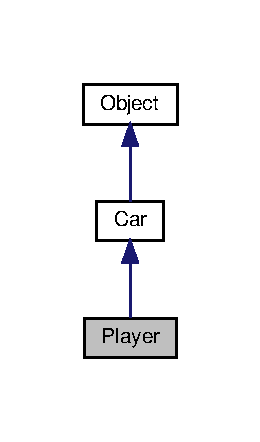
\includegraphics[width=125pt]{classPlayer__inherit__graph}
\end{center}
\end{figure}


Collaboration diagram for Player\+:\nopagebreak
\begin{figure}[H]
\begin{center}
\leavevmode
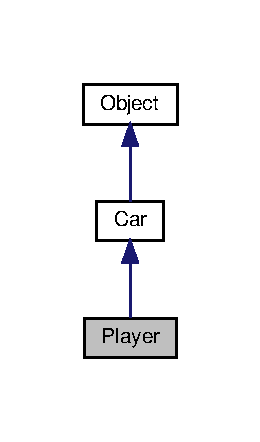
\includegraphics[width=125pt]{classPlayer__coll__graph}
\end{center}
\end{figure}
\subsection*{Public Member Functions}
\begin{DoxyCompactItemize}
\item 
\hyperlink{classPlayer_a502255d0928df823d53f07a0adf5da7e}{Player} (float, float)
\item 
void \hyperlink{classPlayer_a962661bbdff64b195582edbd0dcb3e1e}{car\+Move} (float, float)
\item 
void \hyperlink{classPlayer_a8dded6e745a81ad9f0be87b865856de7}{fire} (std\+::vector$<$ \hyperlink{classBullet}{Bullet} $\ast$$>$ \&, const sf\+::\+Time)
\item 
void \hyperlink{classPlayer_a67f90504cb942a07e98a54b58d4d4a1e}{state\+Checker} (sf\+::\+Time)
\item 
void \hyperlink{classPlayer_a230f0202bf208e5f9c3e0ab54c2c4b15}{fire\+Checker} (sf\+::\+Time)
\item 
float \hyperlink{classPlayer_ab72ff0a99c17ace352a5a44bec0bfa5c}{get\+Player\+Speed} ()
\end{DoxyCompactItemize}
\subsection*{Public Attributes}
\begin{DoxyCompactItemize}
\item 
sf\+::\+Time \hyperlink{classPlayer_a1dd84364f2b6c74be91d6d9cc2430f59}{state\+Time} \{\}
\item 
float \hyperlink{classPlayer_a7b4a4d41e6c36265588539e960f4804f}{multiplier} \{1\}
\item 
bool \hyperlink{classPlayer_ac074e83f791eb282589df6b9456781b7}{state\+Is\+Changed} \{false\}
\end{DoxyCompactItemize}
\subsection*{Additional Inherited Members}


\subsection{Detailed Description}
Class Represents the \hyperlink{classPlayer}{Player} in the game. 

\subsection{Constructor \& Destructor Documentation}
\mbox{\Hypertarget{classPlayer_a502255d0928df823d53f07a0adf5da7e}\label{classPlayer_a502255d0928df823d53f07a0adf5da7e}} 
\index{Player@{Player}!Player@{Player}}
\index{Player@{Player}!Player@{Player}}
\subsubsection{\texorpdfstring{Player()}{Player()}}
{\footnotesize\ttfamily Player\+::\+Player (\begin{DoxyParamCaption}\item[{float}]{pos\+\_\+x,  }\item[{float}]{pos\+\_\+y }\end{DoxyParamCaption})}

Loads the specified sprite for \hyperlink{classPlayer}{Player} and saves it. 

\subsection{Member Function Documentation}
\mbox{\Hypertarget{classPlayer_a962661bbdff64b195582edbd0dcb3e1e}\label{classPlayer_a962661bbdff64b195582edbd0dcb3e1e}} 
\index{Player@{Player}!car\+Move@{car\+Move}}
\index{car\+Move@{car\+Move}!Player@{Player}}
\subsubsection{\texorpdfstring{car\+Move()}{carMove()}}
{\footnotesize\ttfamily void Player\+::car\+Move (\begin{DoxyParamCaption}\item[{float}]{x,  }\item[{float}]{y }\end{DoxyParamCaption})\hspace{0.3cm}{\ttfamily [virtual]}}

Specifik car\+Move funktion 

Implements \hyperlink{classCar_a9650df764ceee00f738b888a7a976996}{Car}.

\mbox{\Hypertarget{classPlayer_a8dded6e745a81ad9f0be87b865856de7}\label{classPlayer_a8dded6e745a81ad9f0be87b865856de7}} 
\index{Player@{Player}!fire@{fire}}
\index{fire@{fire}!Player@{Player}}
\subsubsection{\texorpdfstring{fire()}{fire()}}
{\footnotesize\ttfamily void Player\+::fire (\begin{DoxyParamCaption}\item[{std\+::vector$<$ \hyperlink{classBullet}{Bullet} $\ast$$>$ \&}]{Bullets,  }\item[{const sf\+::\+Time}]{game\+\_\+time }\end{DoxyParamCaption})}

Adds a new \hyperlink{classBullet}{Bullet} to the a bullet vector, and changes fire\+Time to the time parameter. \mbox{\Hypertarget{classPlayer_a230f0202bf208e5f9c3e0ab54c2c4b15}\label{classPlayer_a230f0202bf208e5f9c3e0ab54c2c4b15}} 
\index{Player@{Player}!fire\+Checker@{fire\+Checker}}
\index{fire\+Checker@{fire\+Checker}!Player@{Player}}
\subsubsection{\texorpdfstring{fire\+Checker()}{fireChecker()}}
{\footnotesize\ttfamily void Player\+::fire\+Checker (\begin{DoxyParamCaption}\item[{sf\+::\+Time}]{comp\+\_\+time }\end{DoxyParamCaption})}

Checks if player can fire and changes the can\+Fire bool to true if the player can fire. \mbox{\Hypertarget{classPlayer_ab72ff0a99c17ace352a5a44bec0bfa5c}\label{classPlayer_ab72ff0a99c17ace352a5a44bec0bfa5c}} 
\index{Player@{Player}!get\+Player\+Speed@{get\+Player\+Speed}}
\index{get\+Player\+Speed@{get\+Player\+Speed}!Player@{Player}}
\subsubsection{\texorpdfstring{get\+Player\+Speed()}{getPlayerSpeed()}}
{\footnotesize\ttfamily float Player\+::get\+Player\+Speed (\begin{DoxyParamCaption}{ }\end{DoxyParamCaption})}

Returns player\+\_\+speed float. \mbox{\Hypertarget{classPlayer_a67f90504cb942a07e98a54b58d4d4a1e}\label{classPlayer_a67f90504cb942a07e98a54b58d4d4a1e}} 
\index{Player@{Player}!state\+Checker@{state\+Checker}}
\index{state\+Checker@{state\+Checker}!Player@{Player}}
\subsubsection{\texorpdfstring{state\+Checker()}{stateChecker()}}
{\footnotesize\ttfamily void Player\+::state\+Checker (\begin{DoxyParamCaption}\item[{sf\+::\+Time}]{comp\+\_\+time }\end{DoxyParamCaption})}

Checks if state should still be changed depending on the Time parameter. Changes the state\+Is\+Changed bool to false if the state shouldn\textquotesingle{}t be changed 

\subsection{Member Data Documentation}
\mbox{\Hypertarget{classPlayer_a7b4a4d41e6c36265588539e960f4804f}\label{classPlayer_a7b4a4d41e6c36265588539e960f4804f}} 
\index{Player@{Player}!multiplier@{multiplier}}
\index{multiplier@{multiplier}!Player@{Player}}
\subsubsection{\texorpdfstring{multiplier}{multiplier}}
{\footnotesize\ttfamily float Player\+::multiplier \{1\}}

Players movement multiplier depending on \hyperlink{classBuff__debuff}{Buff\+\_\+debuff} effect \mbox{\Hypertarget{classPlayer_ac074e83f791eb282589df6b9456781b7}\label{classPlayer_ac074e83f791eb282589df6b9456781b7}} 
\index{Player@{Player}!state\+Is\+Changed@{state\+Is\+Changed}}
\index{state\+Is\+Changed@{state\+Is\+Changed}!Player@{Player}}
\subsubsection{\texorpdfstring{state\+Is\+Changed}{stateIsChanged}}
{\footnotesize\ttfamily bool Player\+::state\+Is\+Changed \{false\}}

Represents if the players state is changed \mbox{\Hypertarget{classPlayer_a1dd84364f2b6c74be91d6d9cc2430f59}\label{classPlayer_a1dd84364f2b6c74be91d6d9cc2430f59}} 
\index{Player@{Player}!state\+Time@{state\+Time}}
\index{state\+Time@{state\+Time}!Player@{Player}}
\subsubsection{\texorpdfstring{state\+Time}{stateTime}}
{\footnotesize\ttfamily sf\+::\+Time Player\+::state\+Time \{\}}

Time when state should stop affecting player. 

The documentation for this class was generated from the following files\+:\begin{DoxyCompactItemize}
\item 
car.\+h\item 
car.\+cpp\end{DoxyCompactItemize}

\hypertarget{classScore}{}\section{Score Class Reference}
\label{classScore}\index{Score@{Score}}


{\ttfamily \#include $<$score.\+h$>$}

\subsection*{Public Member Functions}
\begin{DoxyCompactItemize}
\item 
\hyperlink{classScore_a039c99843551e5e4b512ecee99e46617}{Score} ()
\item 
int \hyperlink{classScore_a0edd6880a4747e9ec07751030bdd4689}{get\+\_\+score} ()
\item 
void \hyperlink{classScore_a98e9cf2e21db2a2b0ed2751bb53e8255}{update\+\_\+score} (int)
\item 
void \hyperlink{classScore_a4e4e4e4d043b7b4574827b5a670d55a0}{check\+\_\+time} (sf\+::\+Time)
\item 
void \hyperlink{classScore_a933dc121ad262cd9729f973e02a70cf2}{draw\+Score} (sf\+::\+Render\+Window \&)
\end{DoxyCompactItemize}
\subsection*{Public Attributes}
\begin{DoxyCompactItemize}
\item 
float \hyperlink{classScore_afa64d0ac8f47b5eb21c83d9d1d529877}{count} \{0\}
\end{DoxyCompactItemize}


\subsection{Detailed Description}
This class is responsible for keeping and counting the score when the game is running. 

\subsection{Constructor \& Destructor Documentation}
\mbox{\Hypertarget{classScore_a039c99843551e5e4b512ecee99e46617}\label{classScore_a039c99843551e5e4b512ecee99e46617}} 
\index{Score@{Score}!Score@{Score}}
\index{Score@{Score}!Score@{Score}}
\subsubsection{\texorpdfstring{Score()}{Score()}}
{\footnotesize\ttfamily Score\+::\+Score (\begin{DoxyParamCaption}{ }\end{DoxyParamCaption})}

The constructor creates an sf\+::\+Text object with a the font variable, a set position and color. This is the ingame score counter. 

\subsection{Member Function Documentation}
\mbox{\Hypertarget{classScore_a4e4e4e4d043b7b4574827b5a670d55a0}\label{classScore_a4e4e4e4d043b7b4574827b5a670d55a0}} 
\index{Score@{Score}!check\+\_\+time@{check\+\_\+time}}
\index{check\+\_\+time@{check\+\_\+time}!Score@{Score}}
\subsubsection{\texorpdfstring{check\+\_\+time()}{check\_time()}}
{\footnotesize\ttfamily void Score\+::check\+\_\+time (\begin{DoxyParamCaption}\item[{sf\+::\+Time}]{game\+\_\+time }\end{DoxyParamCaption})}

The bread and butter of this class. This funtion checks if a second has passed and updates the score by one everytime this happens. \mbox{\Hypertarget{classScore_a933dc121ad262cd9729f973e02a70cf2}\label{classScore_a933dc121ad262cd9729f973e02a70cf2}} 
\index{Score@{Score}!draw\+Score@{draw\+Score}}
\index{draw\+Score@{draw\+Score}!Score@{Score}}
\subsubsection{\texorpdfstring{draw\+Score()}{drawScore()}}
{\footnotesize\ttfamily void Score\+::draw\+Score (\begin{DoxyParamCaption}\item[{sf\+::\+Render\+Window \&}]{window }\end{DoxyParamCaption})}

This function draws the score on the screen. \mbox{\Hypertarget{classScore_a0edd6880a4747e9ec07751030bdd4689}\label{classScore_a0edd6880a4747e9ec07751030bdd4689}} 
\index{Score@{Score}!get\+\_\+score@{get\+\_\+score}}
\index{get\+\_\+score@{get\+\_\+score}!Score@{Score}}
\subsubsection{\texorpdfstring{get\+\_\+score()}{get\_score()}}
{\footnotesize\ttfamily int Score\+::get\+\_\+score (\begin{DoxyParamCaption}{ }\end{DoxyParamCaption})}

Getter function that returns the private variable score. \mbox{\Hypertarget{classScore_a98e9cf2e21db2a2b0ed2751bb53e8255}\label{classScore_a98e9cf2e21db2a2b0ed2751bb53e8255}} 
\index{Score@{Score}!update\+\_\+score@{update\+\_\+score}}
\index{update\+\_\+score@{update\+\_\+score}!Score@{Score}}
\subsubsection{\texorpdfstring{update\+\_\+score()}{update\_score()}}
{\footnotesize\ttfamily void Score\+::update\+\_\+score (\begin{DoxyParamCaption}\item[{int}]{add }\end{DoxyParamCaption})}

Function that takes an int as a parameter and adds that int to the score. 

\subsection{Member Data Documentation}
\mbox{\Hypertarget{classScore_afa64d0ac8f47b5eb21c83d9d1d529877}\label{classScore_afa64d0ac8f47b5eb21c83d9d1d529877}} 
\index{Score@{Score}!count@{count}}
\index{count@{count}!Score@{Score}}
\subsubsection{\texorpdfstring{count}{count}}
{\footnotesize\ttfamily float Score\+::count \{0\}}

Public variable that helps to check the time. Every second this variable is being increased by one. Everytime this happens the score is being updated. 

The documentation for this class was generated from the following files\+:\begin{DoxyCompactItemize}
\item 
score.\+h\item 
score.\+cpp\end{DoxyCompactItemize}

\hypertarget{classTurbo}{}\section{Turbo Class Reference}
\label{classTurbo}\index{Turbo@{Turbo}}


{\ttfamily \#include $<$buff\+\_\+debuff.\+h$>$}



Inheritance diagram for Turbo\+:\nopagebreak
\begin{figure}[H]
\begin{center}
\leavevmode
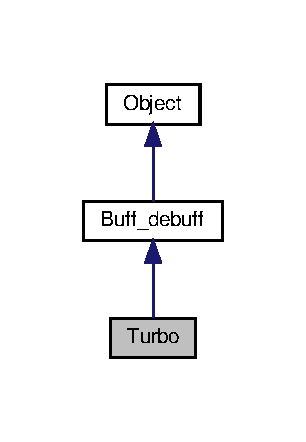
\includegraphics[width=147pt]{classTurbo__inherit__graph}
\end{center}
\end{figure}


Collaboration diagram for Turbo\+:\nopagebreak
\begin{figure}[H]
\begin{center}
\leavevmode
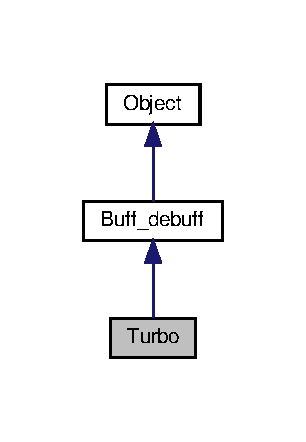
\includegraphics[width=147pt]{classTurbo__coll__graph}
\end{center}
\end{figure}
\subsection*{Public Member Functions}
\begin{DoxyCompactItemize}
\item 
\hyperlink{classTurbo_a11c88626d73b3b4d3462e4b96f4b715c}{Turbo} (float, float)
\end{DoxyCompactItemize}
\subsection*{Additional Inherited Members}


\subsection{Detailed Description}
The turbo class creates a buff object, turbo, that increases the player speed when collided with. 

\subsection{Constructor \& Destructor Documentation}
\mbox{\Hypertarget{classTurbo_a11c88626d73b3b4d3462e4b96f4b715c}\label{classTurbo_a11c88626d73b3b4d3462e4b96f4b715c}} 
\index{Turbo@{Turbo}!Turbo@{Turbo}}
\index{Turbo@{Turbo}!Turbo@{Turbo}}
\subsubsection{\texorpdfstring{Turbo()}{Turbo()}}
{\footnotesize\ttfamily Turbo\+::\+Turbo (\begin{DoxyParamCaption}\item[{float}]{pos\+\_\+x,  }\item[{float}]{pos\+\_\+y }\end{DoxyParamCaption})}

The turbo constructor takes two float parameters, x-\/ and y-\/position(in that order). The constructor then loads the sprite for the turbo object, sets the scale for the sprite, sets the object position to the given parameters and sets the multiplier to two(2). 

The documentation for this class was generated from the following files\+:\begin{DoxyCompactItemize}
\item 
buff\+\_\+debuff.\+h\item 
buff\+\_\+debuff.\+cpp\end{DoxyCompactItemize}

%--- End generated contents ---

% Index
\backmatter
\newpage
\phantomsection
\clearemptydoublepage
\addcontentsline{toc}{chapter}{Index}
\printindex

\end{document}
